%% Version 2022-07-08
%% LaTeX-Vorlage für Abschlussarbeiten
%% Erstellt von Nils Potthoff, ab 2020 erneuert und ausgebaut von Simon Lohmann
%% Lehrstuhl Automatisierungstechnik/Informatik Bergische Universität Wuppertal
%%%%%%%%%%%%%%%%%%%%%%%%%%%%%%%%%%%%%%%%%%%%%%%%%%%%%%%%%%%%%%%%%%%%%%%%%%%%%%%%

%%%%%%%%%%%%%%%%%%%%%%%%%%%%%%%%%%%%%%%%%%%%%
%%% ! WARNUNG ! %%%%%%%%%%%%%%%%%%%%%%%%%%%%%
%%%%%%%%%%%%%%%%%%%%%%%%%%%%%%%%%%%%%%%%%%%%%
%%%  Diese Datei bitte nur bearbeiten,    %%%
%%%   wenn du ein LaTeX-Experte bist      %%%
%%%             U N D                     %%%
%%%  die Vorlage unbedingt ändern willst  %%%
%%%%%%%%%%%%%%%%%%%%%%%%%%%%%%%%%%%%%%%%%%%%%
%%%%%%%%%%%%%%%%%%%%%%%%%%%%%%%%%%%%%%%%%%%%%
%
%%%%%%%%%%%%%%%%%%%%%%%%%%%%%%%%%%%%%%%%%%%%%%%%%%%%%%%%%%%%%%%%%%%%%%%%%%%%%%%%
%%% DATEI-INFO %%%%%%%%%%%%%%%%%%%%%%%%%%%%%%%%%%%%%%%%%%%%%%%%%%%%%%%%%%%%%%%%%
%%%%%%%%%%%%%%%%%%%%%%%%%%%%%%%%%%%%%%%%%%%%%%%%%%%%%%%%%%%%%%%%%%%%%%%%%%%%%%%%
%%% Diese Datei enthält die Titelseite und Standardteile am Anfang der Thesis %%
%%%%%%%%%%%%%%%%%%%%%%%%%%%%%%%%%%%%%%%%%%%%%%%%%%%%%%%%%%%%%%%%%%%%%%%%%%%%%%%%
%
\pagenumbering{Roman}
\pagestyle{plain}
%
% Entscheiden, welches der Logopdfs benutzt wird (verschiedene Schwarztöne)
\newcommand{\buwlogopdf}{Medien/Uni_Wuppertal_Logo__cmykblack.pdf}
\ifbool{color}{%
	\renewcommand{\buwlogopdf}{Medien/Uni_Wuppertal_Logo__richblack.pdf}
}{% color disabled
	\ifstrequal{\colormodel}{rgb}{%
		\renewcommand{\buwlogopdf}{Medien/Uni_Wuppertal_Logo__rgbblack.pdf}
	}{% cmyk/gray/...
		\renewcommand{\buwlogopdf}{Medien/Uni_Wuppertal_Logo__cmykblack}
	}
}
%
%%%%%%%%%%%%%%%%%%%%%%%%%%%%%%%%%%%%%%%%%%%%%%%%%%%%%%%%%%%%%%%%%%%%%%%%%%%%%%%%
%%% Titelseite %%%%%%%%%%%%%%%%%%%%%%%%%%%%%%%%%%%%%%%%%%%%%%%%%%%%%%%%%%%%%%%%%
%
	\begin{titlepage}
		\sffamily%
		%
		\hspace{-1.5em}%
		\includegraphics[width=4.5cm]{\buwlogopdf}%
		\hfill%
		\begin{minipage}[b]{\linewidth-4.5cm}
			\begin{flushright}
				\normalsize{Fakultät für Elektrotechnik,}%
				\\\vspace{0.2mm}
				\normalsize{Informationstechnik und Medientechnik}%
				\vspace*{0.05mm}
			\end{flushright}
		\end{minipage}
		\vspace{-0.3em}
		\begingroup%
			\color{primary}%
			\rule{\textwidth}{3pt}%
		\endgroup%
		\begin{flushright}
			\lehrstuhl
		\end{flushright}
		
		\vspace{3.2em}
		\begin{center}
			\textbf{\Huge{\artderarbeit}}%
			\vspace{1.4em}
			\\
			\textbf{\large{\thema}}%
		\end{center}
		
		
		\vfill
	
	
		\begin{center}
			\Large
			\autor%
			\\
			{\Large\matrikelnummer}%
			\bigskip\\%
			\studiengang%
			\\
			{\large\schwerpunkt}%
			\vspace{2em}%
			\hspace{0em}\\%
			\normalsize%
			\ort, den \abgabedatum%
		\end{center}
		
		
		\vspace{7.5em}
		
		
		\pbox[t][2em]{\linewidth}{Betreuer}%
		\quad%
		\pbox[t][2em]{\linewidth}{\betreuer}%
		\hfill%
		\pbox[t][2em]{\linewidth}{Erstgutachter\\Zweitgutachter}%
		\quad%
		\pbox[t][2em]{\linewidth}{\prueferA\\\prueferB}%
	
	\end{titlepage}
	\ifbool{doppelseitig}{%
		% im doppelseitigen Modus zählt report wie gewünscht
	}{%
		\stepcounter{page}% Seite manuell hochzählen, weil report das im einseitigen Modus nicht macht, im doppelseitigen aber schon (Konsistenz)
	}
	\clearpage{\pagestyle{empty}\cleardoublepage}
%
%
%%%%%%%%%%%%%%%%%%%%%%%%%%%%%%%%%%%%%%%%%%%%%%%%%%%%%%%%%%%%%%%%%%%%%%%%%%%%%%%%
%%% Themenblatt / Aufgabenstellung %%%%%%%%%%%%%%%%%%%%%%%%%%%%%%%%%%%%%%%%%%%%%
%
	\pdfbookmark[1]{Aufgabenstellung}{aufgabe}%
	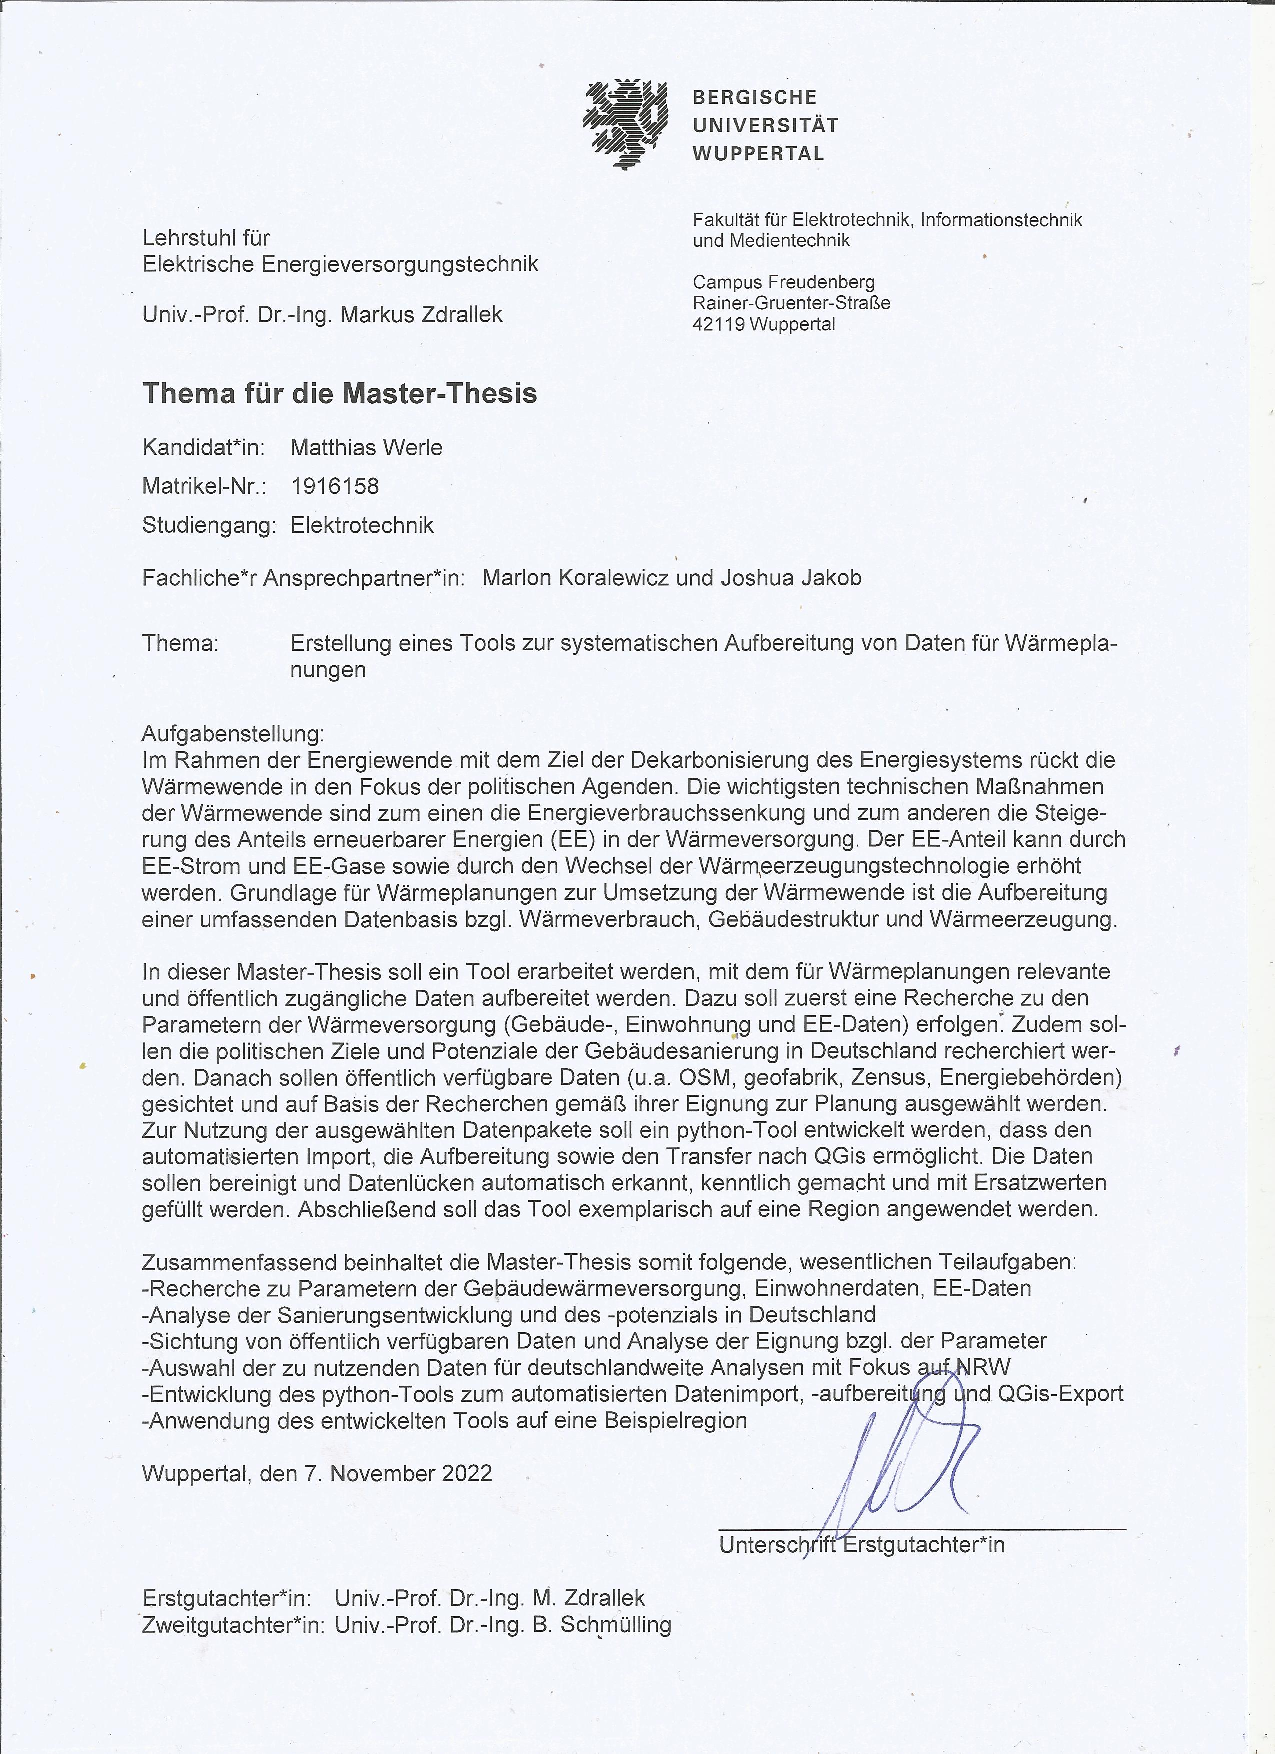
\includepdf[
		pages={1},
		fitpaper=true
	]{Medien/own/Aufgabenstellung_S1.pdf}%
	
\includepdf[
	pages={1},
	fitpaper=true
	]{Medien/own/Aufgabenstellung_S2.pdf}%
	\clearpage{\pagestyle{empty}\cleardoublepage}%
%
%
%%%%%%%%%%%%%%%%%%%%%%%%%%%%%%%%%%%%%%%%%%%%%%%%%%%%%%%%%%%%%%%%%%%%%%%%%%%%%%%%
%%% Verlängerung %%%%%%%%%%%%%%%%%%%%%%%%%%%%%%%%%%%%%%%%%%%%%%%%%%%%%%%%%%%%%%%
%
	\ifbool{verlaengerung}{%
		\cleardoublepage%
		\pdfbookmark[1]{Verlängerung}{verlaengerung}%
		\includepdf[pages={1},fitpaper=true]{Medien/Verlaengerung.pdf}%
	  	\clearpage{\pagestyle{empty}\cleardoublepage}%
	}{}%
%
%
%%%%%%%%%%%%%%%%%%%%%%%%%%%%%%%%%%%%%%%%%%%%%%%%%%%%%%%%%%%%%%%%%%%%%%%%%%%%%%%%
%%% Erklärungen %%%%%%%%%%%%%%%%%%%%%%%%%%%%%%%%%%%%%%%%%%%%%%%%%%%%%%%%%%%%%%%%
%
	\pdfbookmark[1]{Erklärungen}{erklaerung}%
	\vspace*{2em}%
	\section*{Eidesstattliche Erklärung}%
	% original
	%\noindent Hiermit versichere ich, dass ich die Arbeit selbstständig verfasst, keine anderen als die angegebenen Quellen und Hilfsmittel benutzt sowie Zitate kenntlich gemacht habe.%
	% eigen
	\noindent Hiermit versichere ich, dass ich die Arbeit selbstständig verfasst, ChatGPT\footnote{Chatbot von OpenAI, verschiedene Versionen} lediglich sowohl als Ideen bzw. Rat gebende KI als auch als Einschätzungstool und keine anderen als die angegebenen Quellen und Hilfsmittel benutzt sowie Zitate kenntlich gemacht habe.
	
	\ifbool{zusatzErklaerung}{\vfill}{\vspace{4em}}%
	\begin{tabular}{lc}%
	\ort, den \abgabedatum \hspace*{1cm}& \rule[2px]{5cm}{0.5px}\\%
	                                    &\footnotesize{(Unterschrift)}%
	\end{tabular}
	\ifbool{zusatzErklaerung}{\vfill}{\vspace{5em}}%
	
	\section*{Einverständniserklärung}
	% original
	%\noindent Ich bin damit einverstanden, dass meine Abschlussarbeit wissenschaftlich interessierten Personen oder Institutionen zur Verfügung gestellt werden kann. Korrektur- oder Bewertungshinweise in meiner Arbeit dürfen nicht zitiert werden.
	% eigen
	\noindent Ich bin damit einverstanden, dass meine Arbeit unter einer Creative Commons
	Attribution-NonCommercial-ShareAlike 4.0 International License (CC BY-NC-SA
	4.0) lizensiert veröffentlicht wird. Unter Einhaltung der Lizenzgebühren, kann die-
	se Arbeit unter gleichen Bedingungen geteilt und verändert werden. Die Arbeit darf
	somit elektronisch gespeichert, in andere Formate konvertiert, auf den Servern der
	Bergischen Universität Wuppertal öffentlich zugänglich gemacht und über das Internet ver-
	breitet werden. Ausgeschlossen hiervon sind Korrektur- und Bewertungshinweise in meiner Arbeit. Korrektur- und Bewertungshinweise in meiner Arbeit dürfen nicht zitiert werden.
	
	\ifbool{zusatzErklaerung}{\vfill}{\vspace{4em}}%
	\begin{tabular}{lc}
	\ort, den \abgabedatum \hspace*{1cm}& \rule[-2px]{5cm}{0.5px} \\ 
	                                       &\footnotesize{(Unterschrift)}
	\end{tabular}
	\ifbool{zusatzErklaerung}{%
		\vfill
		%% Version 2022-07-08
%% LaTeX-Vorlage für Abschlussarbeiten
%% Erstellt von Nils Potthoff, ab 2020 erneuert und ausgebaut von Simon Lohmann
%% Lehrstuhl Automatisierungstechnik/Informatik Bergische Universität Wuppertal
%%%%%%%%%%%%%%%%%%%%%%%%%%%%%%%%%%%%%%%%%%%%%%%%%%%%%%%%%%%%%%%%%%%%%%%%%%%%%%%%

% Falls weitere Erklärungen gewünscht sind,
% können diese HIER eingefügt werden:
%
% Dies ist z.B. für den Fall gedacht, das eure Prüfungsordnung eine zusätzliche Erklärung einfordert...
%	
	\section*{Risikoaufklärung: \textit{Konsum von Text}} % Titel der Erklärung
	
	% Text der Erklärung:
	Dieses Beispiel enthält \emph{Text}. Der regelmäßige Konsum von hochkonzentriertem \emph{Text} kann unter Umständen Nebenwirkungen wie z.\,B. akuten Informationsgewinn, gesteigerte Redegewandheit oder verbesserten Satzbau zur Folge haben. Sofern Sie dies nicht beabsichtigen, hinterfragen Sie Ihre Motivation zu Studieren und/oder wenden Sie sich an eine entsprechende Beratungsstelle.
	\\
	
	
	{%
		\hrule
		\vspace{0.2em}
		\footnotesize%
		\sffamily%
		\noindent
		\textbf{Zu Risiken und Nebenwirkungen fragen Sie nicht Ihren Arzt oder Apotheker.}\\Dessen Wissen bezüglich Ihrer Thesisaktivitäten verhält sich zu Ihren Kentnissen I.d.R. orthogonal, d.h. es kann kein Zusammenhang hergeleitet werden. Der Erwartungswert der Verwirrtheit des Angesprochenen ergibt sich folglich aus dem reziproken Bekanntheitsgrad Ihrer Thesisaktivitäten reduziert um frühere Thesisaktivitäten des Angesprochenen.
		\hrule
	}~
	\\
	
	\noindent
	Ich habe die Risikoaufklärung zun möglichen Nebenwirkungen des Konsums von \emph{Text} gelesen\footnote{Gehen Sie weiter. Es gibt hier nichts zu sehen!} und akzeptiere die Möglichkeit eines ggf. unbeabsichtigten Wissensgewinns bei meiner Recherche.
	
	
	% Datum + Unterschrift-Feld (hier müsst Ihr normalerweise nichts ändern):
	\vfill
	\begin{tabular}{l c}
		\ort, den \abgabedatum \hspace*{1cm}& \rule[-2px]{5cm}{0.5px} \\ 
		&\footnotesize{(Unterschrift)}
	\end{tabular}

		\vfill
	}{}

	\begin{figure}[h]
		
\includegraphics[width=0.2\linewidth]{./Medien/own/cc_by_nc_sa.png}
	\end{figure}

	\clearpage	
%
%
%%%%%%%%%%%%%%%%%%%%%%%%%%%%%%%%%%%%%%%%%%%%%%%%%%%%%%%%%%%%%%%%%%%%%%%%%%%%%%%%
%%% Danksagung %%%%%%%%%%%%%%%%%%%%%%%%%%%%%%%%%%%%%%%%%%%%%%%%%%%%%%%%%%%%%%%%%
	\ifbool{danksagung}{%
		\vspace*{\fill}\vspace{-3em}%
		\pdfbookmark[1]{Danksagung}{danksagung}%
		%% Version 2022-07-08
%% LaTeX-Vorlage für Abschlussarbeiten
%% Erstellt von Nils Potthoff, ab 2020 erneuert und ausgebaut von Simon Lohmann
%% Lehrstuhl Automatisierungstechnik/Informatik Bergische Universität Wuppertal
%%%%%%%%%%%%%%%%%%%%%%%%%%%%%%%%%%%%%%%%%%%%%%%%%%%%%%%%%%%%%%%%%%%%%%%%%%%%%%%%

%\section*{Danksagung}
%\todo{Text der Danksagung wird hier eingetragen.}

%Lorem ipsum dolor sit amet, consectetur adipiscing elit. Integer libero erat, tincidunt quis molestie nec, ultrices nec felis. Cras tincidunt tempor sapien ac cursus. Pellentesque habitant morbi tristique senectus et netus et malesuada fames ac turpis egestas. Nunc eu magna ut sem condimentum posuere. Nulla ullamcorper sapien et sem placerat in blandit libero tempor. Pellentesque non justo in arcu porta lacinia non eget massa. Integer vel lectus sed ipsum sagittis mollis. Cras congue, orci et suscipit tristique, enim metus congue ante, et adipiscing neque justo eget mi. Aliquam ut ligula tortor, eu commodo ante. Nam faucibus lorem ultricies metus suscipit cursus. Maecenas adipiscing convallis felis, mattis sollicitudin sapien aliquam eget. Vivamus cursus mattis massa id scelerisque. Quisque dolor tellus, bibendum in adipiscing in, imperdiet vel augue. Fusce posuere lacus vel neque molestie in congue leo ultrices.
%
		\vfill%
	}{}
%
%
%%%%%%%%%%%%%%%%%%%%%%%%%%%%%%%%%%%%%%%%%%%%%%%%%%%%%%%%%%%%%%%%%%%%%%%%%%%%%%%%
%%% Kurzfassung & Abstract %%%%%%%%%%%%%%%%%%%%%%%%%%%%%%%%%%%%%%%%%%%%%%%%%%%%%
%
	\clearpage{\pagestyle{empty}\cleardoublepage}
	\vspace*{\fill}\vspace{-3em}
	\pdfbookmark[1]{Kurzfassung}{kurzfassung}
	%% Version 2022-07-08
%% LaTeX-Vorlage für Abschlussarbeiten
%% Erstellt von Nils Potthoff, ab 2020 erneuert und ausgebaut von Simon Lohmann
%% Lehrstuhl Automatisierungstechnik/Informatik Bergische Universität Wuppertal
%%%%%%%%%%%%%%%%%%%%%%%%%%%%%%%%%%%%%%%%%%%%%%%%%%%%%%%%%%%%%%%%%%%%%%%%%%%%%%%%

% INFO: Die Kurzfassung wird immer auf Deutsch UND Englisch benötigt!

% Kurzfassung auf Deutsch
\begingroup 
	\selectlanguage{ngerman}% der folgende Text ist auf Deutsch
	\section*{Kurzfassung}
	% Intro
	Die Wärmewende mit den Ziel der Dekarbonisierung des Wärmesektors ist integraler Bestandteil der Energiewende zur Erreichung klimaneutraler Energiesysteme. Die Dekarbonisierung des Wärmesektors kann zum Einen durch die Senkung des Wärmeverbrauchs und zum Anderen durch die Steigerung des Anteils Erneuerbarer Energien bei der Wärmeerzeugung erreicht werden. Zur Umsetzung beider Optionen bietet sich eine Vielzahl technischer Maßnahmen an. Welche Maßnahmen sich je nach lokalen Begebenheiten am besten eignen, lässt sich durch Wärmeplanungen bestimmen. Mittels einer Bestandsaufnahme, Potentialanalysen und Aufstellungen von Zielszenarien wird eine lokale Wärmewendestrategie zur Erreichung der gesetzten Ziele entwickelt. Hierfür bedarf es einer umfassenden Datengrundlage u.a. bezüglich der Gebäudestruktur, des Wärmeverbrauchs und der Wärmeerzeugung. 
	
	% Ziel: Daten sichten, auswählen, Tool entwickeln; Daten für D. mit Fokus auf NRW
	Ziel dieser Thesis ist die Sichtung öffentlich verfügbarer Daten, Auswahl geeigneter Daten für Wärmeplanungen und die Erstellung eines Python-Tools zur systematischen Aufbereitung der ausgewählten Daten für den Export nach QGIS. 
	
	% Datengrundlage
	Als Datengrundlage wurden Datensätze für Basis-Layer, Gebäudestruktur, Wärme-Erzeugung und Wärme-Verbräuchen von Wohngebäuden gewählt. Zu den verwendeten Datensätzen gehören Amtliche Basiskarten, OpenStreetMap Daten, Digitale Verwaltungsgrenzen von Gemeinden, ALKIS-Hausumringe, Zensus Gebäude-, Wohnungs- und Einwohnungsdaten, Schutzgebiete der Landschaftsinformationssammlung des LANUV, Energie-Erzeugungs-Anlagen Standorten des LANUV inklusive Standorten mit KWK-Relevanz und Industrieller Abwärme sowie Raumwärmebedarfs-Modelle des LANUV.

	% Tool
	Es wurde ein Python-Tool entwickelt, welches modular für alle genannten Datensätze anwendbar ist. Die ausgewählten Datensätze werden automatisch räumlich zugeschnitten, anhand einstellbarer Filter auf gewünschte Merkmale (Zensus) oder Energieträger (Erzeugungs-Anlagen Standorte) reduziert und für die Nutzung in QGIS aufbereitet z.B. durch Reformatierung oder Georeferenzierung.
	
	Darüber hinaus können Synthese-Datensätze erstellt werden. Diese sind zum Einen Zensus-Merkmal-Ausprägungen (z.B. Baualtersklassen) zugewiesene ALKIS-Hausumringen und zum Anderen aggregierte estimierte Wärmeverbräuche des Raumwärmebedarfs-Modell des LANUV in einstellbaren Sub-Arealen. Daraus abgeleitet werden spezifische Wärmeverbräuche je Flächeneinheit und Jahr einzelner Sub-Areale als Indikator für die Eignung von Wärmenetzen. Als Sub-Areale können INSPIRE-konformen Gitterzellen, Baublöcken einer Gemeinde, Quartiere, Stadtteile oder beliebige Polygone verwendet werden.
	
	Optional können auto-generierte Pre-Analyse-Dateien mit statistischen Auswertungen im .csv-Format erstellt werden. Diese umfassen u.a. Häufigkeits-Verteilungen von Zensus Merkmals-Ausprägungen im originalen, zugeschnittenen Zensus-Datensatz sowie im erstellbaren Synthese-Datensatzes aus Zensus-Gebäudedaten und ALKIS-Hausumringen. 
	
	Für die Darstellung der aufbereiteten Daten in QGIS wurden Layer-Style-Definitionen im Github-Repository dieser Arbeit gemeinsam mit dem Python-Tool und der Thesis zum Download bereit gestellt. 
	
	Exemplarisch wurde das Tool auf eine Beispielregion um die eingestellten Gemeinden Wuppertal, Velbert und Solingen hin angewandt. Die aufbereiteten Daten für die Region wurden in QGIS visualisiert und exemplarisch analysiert. 
	
\endgroup

% Kurzfassung auf Englisch
\begingroup
	\selectlanguage{english}% der folgende Text ist auf Englisch
	\section*{Abstract}
	The sustainable heat transition with the aim to decarbonise the heat sector is integral part of the sustainable energy transition to reach climate-neutral energy systems. The decarbonisation of the heat sector can on the one hand reached by lowering the heat consumption on the other hand by raising the share of renewable energies in the heat generation. For the realisation of both options exist plenty of technological methods. Which one is the best according to indivudal local conditions can be determined by heat plans (Wärmeplanungen). Based on analysis of the status-quo and potentials aswell as set-up target scenarios local sustainable heat transition strategies are developped. An extensive data base is therefor needed e.g. regarding the composition of buildings, the heat consomption and the heat generation.
	
	The aim of this thesis on the one hand is to search and select useful data for heat planning and on the other hand to develop a python-tool for systematic preparation of the chosen data for an export to QGIS. 
	
	As data base were data sets chosen for base layers, composition of buildings, heat generation and heat consumption in residential buildings. The chosen data sets are official base maps (Amtliche Basiskarten), OpenStreetMap data, digital administrative borders of municipalities (Digitale Verwaltungsgrenzen), ALKIS house footprints (ALKIS-Hausumringe), Zensus building, flat and population data (Zensus Gebäude-, Wohnungs- und Einwohnungsdaten), protected areas of the landscapes information collection (Landschaftsinformationssammlung) of LANUV, energy generation units positions (Energie-Erzeugungs-Anlagen standorte) including positions of combined heat and power generation relevance and industrial waste heat (Standorte mit KWK-Relevanz und Industrieller Abwärme) as well as space heating demand models (Raumwärmebedarfs-Modelle) of LANUV.
	
	The developed python tool can modularly applied on each mentioned data set. The chosen data sets are automatically spatially cropped, reduced according to settable filters for desired features (Zensus) or energy sources (energy generation units positions) and prepared for usage in QGIS e.g. by reformatting or georeferencing.
	
	More over synthesis data sets can be created. One is modified ALKIS house footprints with alloted Zensus building feature characteristics (e.g. construction age classes). The other one are modified sub areas with aggregated estimated heat consumptions from the heat space heating demand model of LANUV. Hence specific heat consumptions per square meter and year are derived for each sub area as an indicator for the suitability of heat grids. Sub areas can be chosen at will e.g. city blocks, urban quarters, urban districts or any kind of polygons. 
	
	Optinally it is possible to create auto-generated pre-analysis files in .csv-format for statistical analyses. These include among others the incidence of occurring Zensus feature characteristics both in the original Zensus building dataset and in the synthesis data set derived from the Zensus building dataset and the ALKIS house footprints dataset. 
	
	To display the preprocessed data in QGIS layer style definitions are made available in the github repository of this work together with the python tool and the thesis.
	
	Exemplarily the tool was applied on a sample region around the preset municipalities Wuppertal, Velbert and Solingen. The preprocessed data was visualised in QGIS and exemplarily analysed.
\endgroup

	\vfill
	\clearpage
%
%
%%%%%%%%%%%%%%%%%%%%%%%%%%%%%%%%%%%%%%%%%%%%%%%%%%%%%%%%%%%%%
%  INHALTSVERZEICHNIS
\markboth{\contentsname}{}
\pdfbookmark[1]{\contentsname}{toc}
\begingroup
	\renewcommand{\markboth}[2]{}{}
	\tableofcontents
\endgroup
\clearpage
%
%
%%WIDMUNG, VORWORT
%
%\nomenclature{$x$}{Description}
%\nomenclature{TEXT}{Abkürz}
%% Ende der Titelei; es folgt der Hauptteil
\ifbool{doppelseitig}{%
	\clearpage%
	\hphantom{anker, damit hier auch wirklich eine leere Seite ist}%
}{}%
{\pagestyle{empty}\cleardoublepage}% Inhalt soll auf rechter Seite beginnen
\pagenumbering{arabic}%
\pagestyle{thesis-page-regular}%
